\section{Progress in preparation for installation}
\label{sec:EPProg}

The energy plane has been installed in the NEW apparatus. Figure \ref{fig:energy_installation} shows different stages of the installation process. The most relevant steps were:
\begin{itemize}
\item The copper support plate (mother-can) has been installed in NEW vessel.
\item 14 sapphire windows have been successfully brazed to their copper window frames. 12 windows are properly installed in the mother can.
\item 14 sapphire windows have been coated with PEDOT using spin coating technique at the ICMol facilities.
\item 14 sapphire windows have been coated with TPB.
\item PMTs have been cabled up to the DAQ.
\item The PMT bases have been potted into their copper heat sinks using epoxy.
\item The PMT bases have been tested inside the detector.
\end{itemize}


\begin{figure}
  \begin{center}
    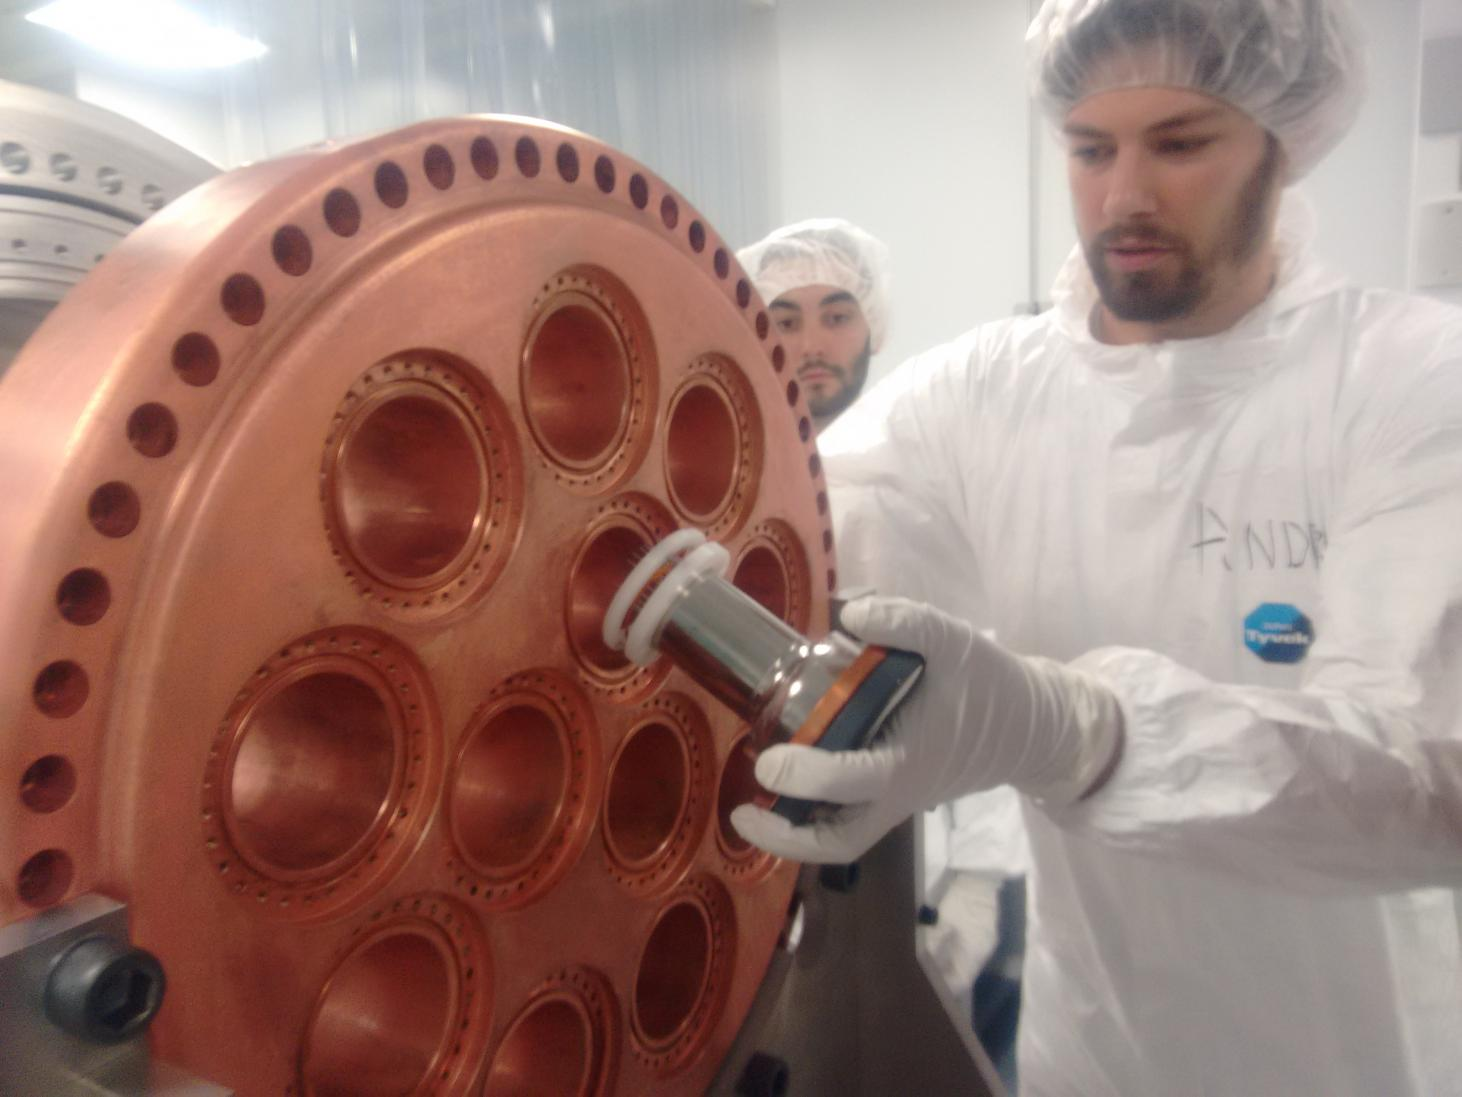
\includegraphics[height=4cm,width=0.45\textwidth]{img/Andrew_pmt.jpg}
	  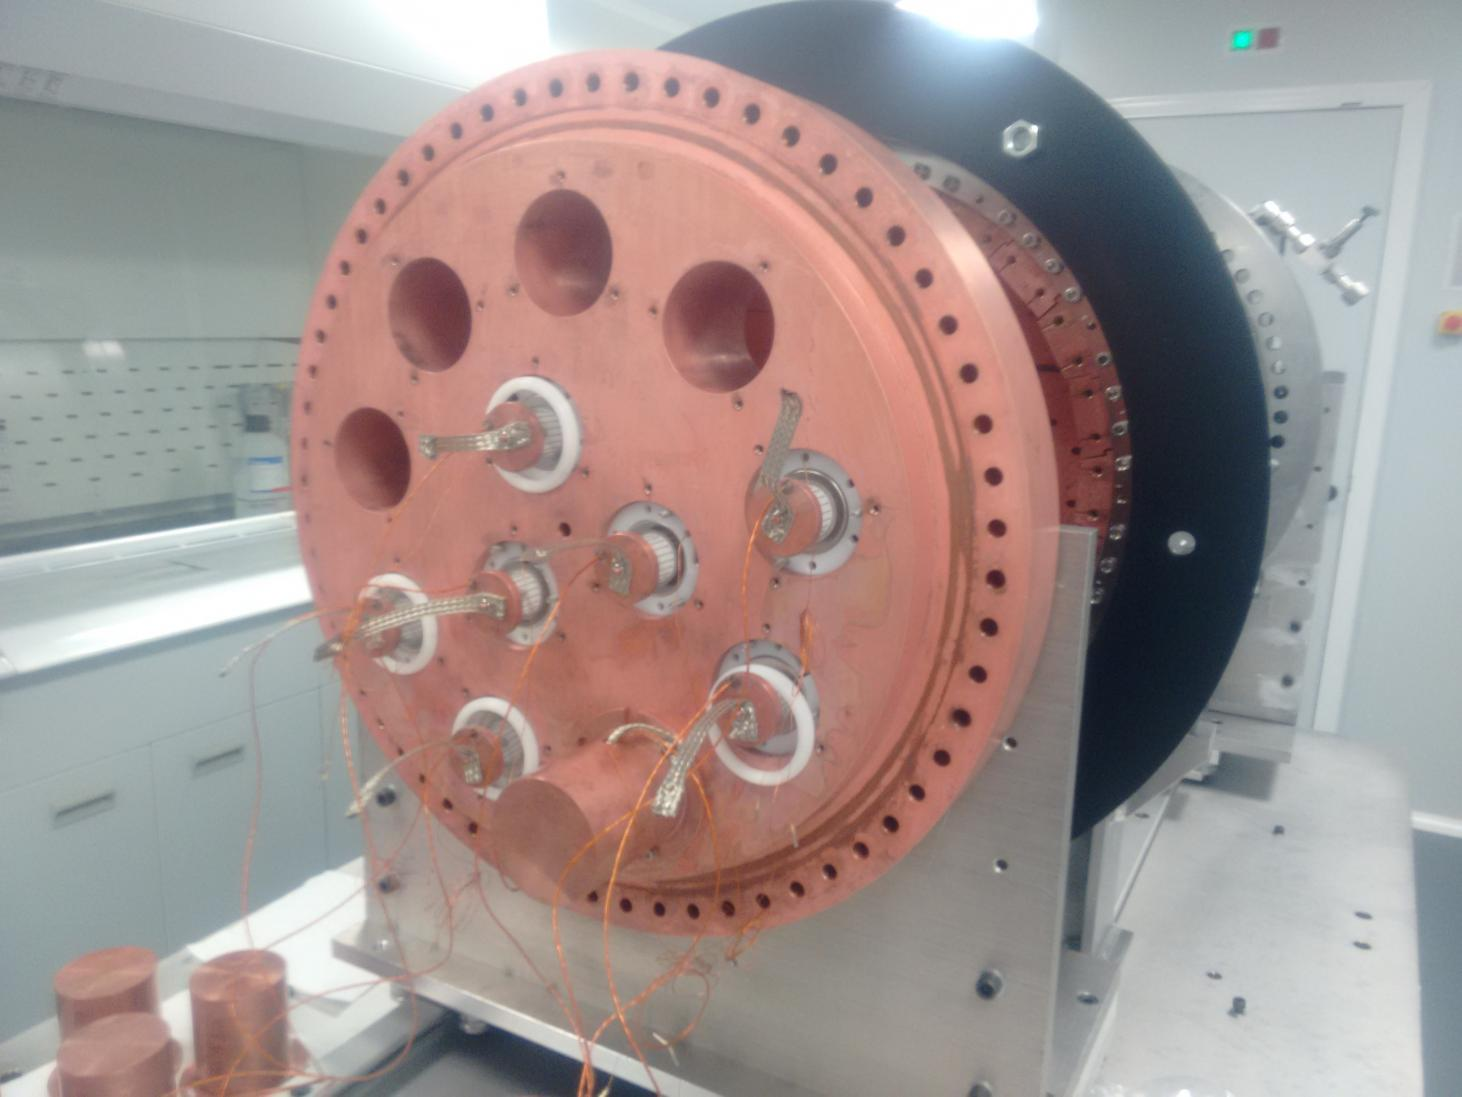
\includegraphics[height=4cm,width=0.45\textwidth]{img/PMTsback}
    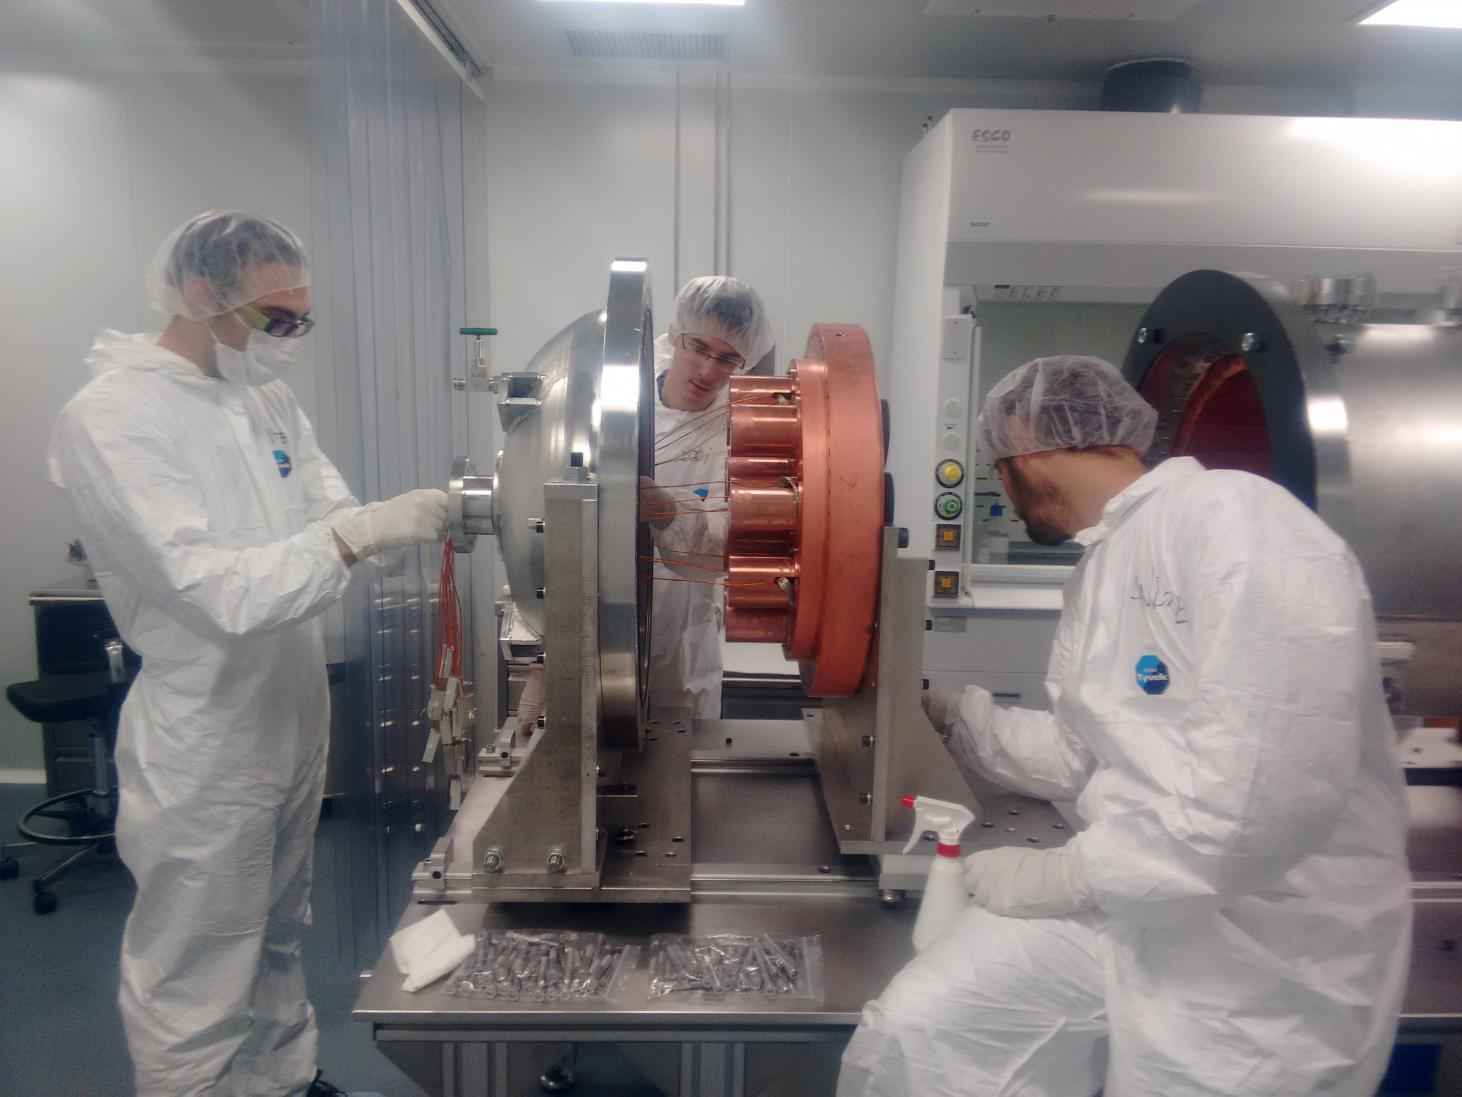
\includegraphics[height=4cm,width=0.45\textwidth]{img/cabling}
	 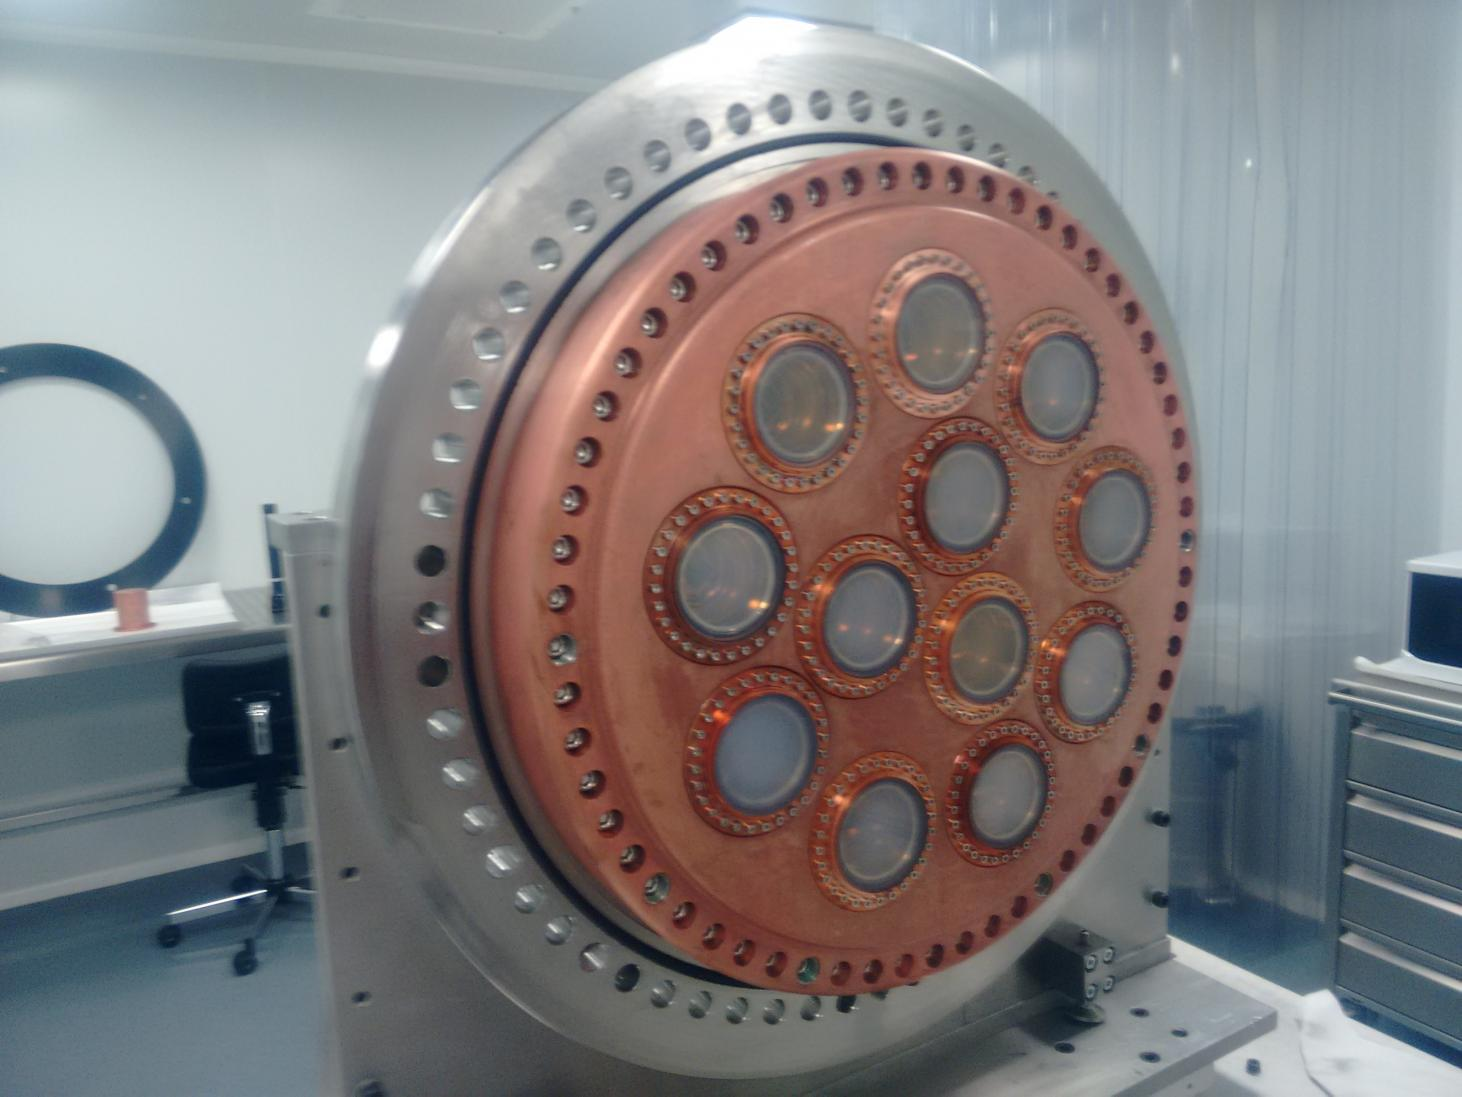
\includegraphics[height=4cm,width=0.45\textwidth]{img/full_energyplane} \\
	  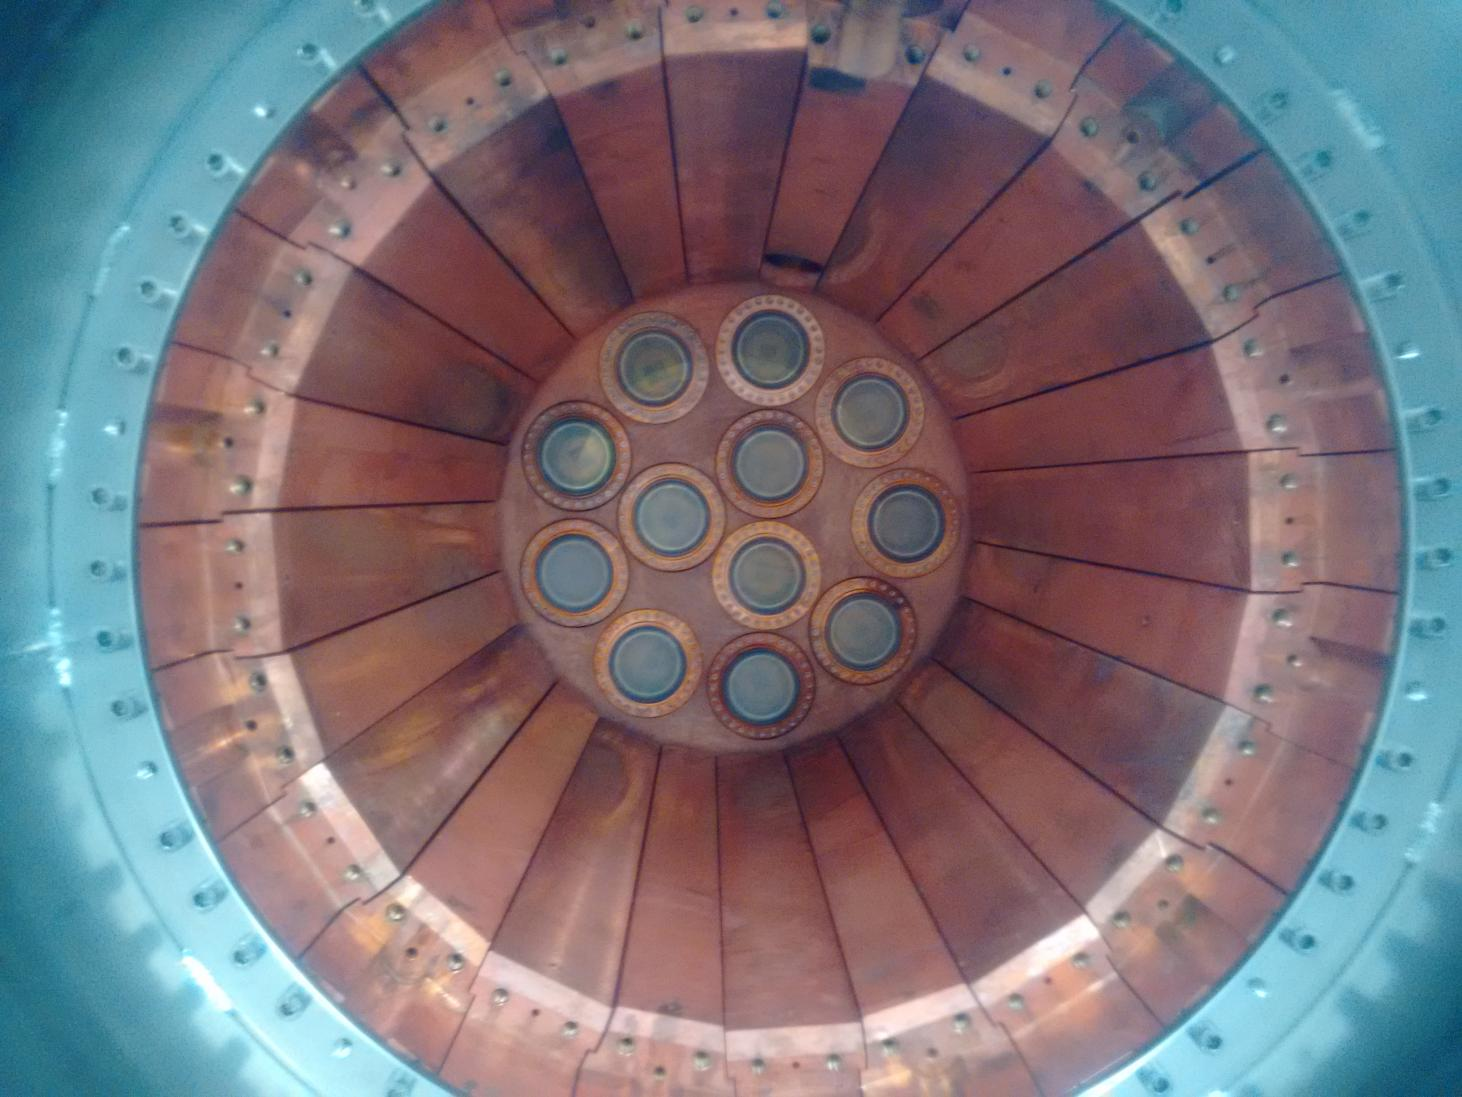
\includegraphics[height=4cm,width=0.45\textwidth]{img/full_energyplane_closed}
  \end{center}
  \caption{Different stages of the installation of the energy plane: Top left picture shows the positioning of the PMTs inside the mother can. Top right shows the back side of the mother can before the copper shielding for the PMTs is added. The copper hat covering the PMTs bases with the thermal contact cable is visible. Middle left shows the process of cabling and labelling the different PMTs. Middle right shows the energy plane once installed. The last picture, bottom, shows energy plane once the end-cap is closed.}
  \label{fig:energy_installation}
\end{figure}
